\chapter{PHÂN TÍCH DỮ LIỆU VỚI HỌC MÁY VÀ ĐỐI SÁNH KẾT QUẢ}
\label{ch:chuong5}

\startcontents[chapters]
\printmyminitoc{
Chương này sử dụng trực tiếp các phiên bản dữ liệu đã làm sạch ở Chương 4 (mục 4.1, 4.3) làm đầu vào cho ba bài toán học máy kinh điển: phân lớp (Classification) trên dữ liệu Nhóm A, hồi quy chuỗi thời gian (Regression) trên dữ liệu Nhóm B, và gom cụm (Clustering) không giám sát trên cả ba nhóm dữ liệu A, B, C. Mục tiêu không chỉ là tối ưu chỉ số hiệu năng mà còn diễn giải ý nghĩa thực tế của kết quả, đặc biệt là ảnh hưởng của các đặc điểm dữ liệu đã phát hiện ở Chương 4 (mất cân bằng lớp, outlier, tính mùa vụ...) lên hành vi của mô hình.}

\section{Môi trường cài đặt và cách đánh giá}

\subsection{Thiết lập môi trường thực nghiệm}

Toàn bộ thực nghiệm được cài đặt bằng \textbf{Python 3}, sử dụng các thư viện chính: \texttt{pandas}/\texttt{numpy} (xử lý dữ liệu), \texttt{scikit-learn} (Logistic Regression, Random Forest, SVM, KMeans, Agglomerative Clustering, Gaussian Mixture, các độ đo đánh giá và \texttt{StandardScaler}), \texttt{statsmodels} (ARIMA), \texttt{xgboost} (XGBoost Regressor), \texttt{matplotlib}/\texttt{seaborn} (trực quan hóa kết quả). Dữ liệu đầu vào là các phiên bản \textbf{đã làm sạch} (đã điền khuyết, xử lý outlier) được xuất ra từ Chương 4, đảm bảo tính nhất quán giữa bước phân tích khám phá dữ liệu và bước huấn luyện mô hình.

Quy trình thực nghiệm được tổ chức thành 5 script độc lập, tương ứng với từng bước của pipeline:
\begin{itemize}
    \item \texttt{step1\_classification.py} -- huấn luyện và đánh giá 3 thuật toán phân lớp trên 3 bộ dữ liệu Nhóm A;
    \item \texttt{step2\_confusion\_and\_imbalance.py} -- dựng ma trận nhầm lẫn và phân tích chuyên sâu vấn đề mất cân bằng lớp trên CDC Diabetes;
    \item \texttt{step3\_regression.py} -- huấn luyện 3 mô hình dự báo chuỗi thời gian trên Appliances Energy;
    \item \texttt{step4\_regression\_charts.py} -- dựng các biểu đồ phân tích dự báo (forecast, residual, feature importance);
    \item \texttt{step5\_clustering.py} -- thực hiện gom cụm không giám sát trên 3 bộ dữ liệu đại diện Nhóm A/B/C.
\end{itemize}

\subsection{Các độ đo đánh giá}

Đối với bài toán \textbf{phân lớp} (mục~\ref{sec:classification}), các độ đo được sử dụng gồm Accuracy, Precision, Recall và F1-Score (tính theo kiểu binary cho bài toán 2 lớp, và macro-average cho bài toán 3 lớp CDC Diabetes để tránh chỉ số bị chi phối bởi lớp đa số):

\begin{equation}\label{eq:acc}
Accuracy = \frac{TP+TN}{TP+TN+FP+FN}
\end{equation}

\begin{equation}
Precision = \frac{TP}{TP+FP}
\end{equation}

\begin{equation}
Recall = \frac{TP}{TP+FN}
\end{equation}

\begin{equation}
F1 = \frac{2 \times Precision \times Recall}{Precision+Recall} = \frac{2 \times TP}{2 \times TP+FP+FN}
\end{equation}

Đối với bài toán \textbf{hồi quy} (mục~\ref{sec:regression}), sử dụng MAE (Mean Absolute Error), RMSE (Root Mean Squared Error) và MAPE (Mean Absolute Percentage Error):

\begin{equation}
MAE = \frac{1}{n}\sum_{i=1}^{n}|y_i - \hat{y}_i\,|, \quad
RMSE = \sqrt{\frac{1}{n}\sum_{i=1}^{n}(y_i - \hat{y}_i)^2}, \quad
MAPE = \frac{100\%}{n}\sum_{i=1}^{n}\left|\frac{y_i - \hat{y}_i}{y_i}\right|
\end{equation}

Đối với bài toán \textbf{gom cụm} (mục~\ref{sec:clustering}), sử dụng Silhouette Score (đo mức độ tách biệt giữa các cụm, dao động từ $-1$ đến $1$, càng gần 1 càng tốt) làm tiêu chí chính để chọn số cụm $K$ tối ưu và so sánh giữa các giải thuật.


\section{Bài toán dự đoán phân lớp (Classification) trên Data A}
\label{sec:classification}

Ba bộ dữ liệu Nhóm A đã được làm sạch ở Chương 4 được sử dụng làm ba bài toán phân lớp độc lập, mỗi bài toán ứng với một biến mục tiêu (target) khác nhau:
\begin{itemize}
    \item \textbf{Target 1 -- Breast Cancer Wisconsin}: phân lớp nhị phân \texttt{diagnosis} (Benign/Malignant), dữ liệu đầu vào là 6 đặc trưng hình thái đã làm sạch ở mục 4.1.1 (569 mẫu);
    \item \textbf{Target 2 -- Heart Disease (Cleveland)}: phân lớp nhị phân \texttt{target} (Có/Không bệnh tim), 13 đặc trưng lâm sàng đã làm sạch ở mục 4.1.2 (303 mẫu);
    \item \textbf{Target 3 -- CDC Diabetes Health Indicators}: phân lớp \textbf{3 mức} \texttt{Diabetes\_012} (Không tiểu đường/Tiền tiểu đường/Tiểu đường), 21 đặc trưng đã làm sạch ở mục 4.1.3.
\end{itemize}

\subsection{Quy trình thực nghiệm}

Quy trình áp dụng thống nhất cho cả 3 bộ dữ liệu:
\begin{enumerate}
    \item \textbf{Chia tách Train/Test}: tỉ lệ 80/20, sử dụng \texttt{stratify} theo biến mục tiêu để đảm bảo tỉ lệ các lớp trong tập train và test tương đồng với tỉ lệ gốc -- đặc biệt quan trọng với bộ CDC Diabetes vốn đã mất cân bằng lớp nghiêm trọng (Chương 4, mục 4.1.3).
    \item \textbf{Chuẩn hóa dữ liệu}: áp dụng \texttt{StandardScaler} (đưa về trung bình 0, phương sai 1) cho Logistic Regression và SVM (2 thuật toán nhạy cảm với thang đo); Random Forest giữ nguyên dữ liệu gốc vì thuật toán dựa trên cây quyết định không yêu cầu chuẩn hóa.
    \item \textbf{Xử lý mất cân bằng lớp}: tham số \texttt{class\_weight="balanced"} được kích hoạt cho Random Forest và SVM, tự động tăng trọng số cho các lớp thiểu số trong hàm mất mát.
    \item \textbf{Riêng bộ CDC Diabetes} (253.680 mẫu): do kích thước quá lớn khiến SVM không khả thi về thời gian huấn luyện, nhóm lấy mẫu ngẫu nhiên phân tầng (stratified subsample) 30.000 dòng (giữ nguyên tỉ lệ 3 lớp gốc) trước khi chia Train/Test, một điều chỉnh thực tế thường gặp khi triển khai SVM trên dữ liệu lớn.
\end{enumerate}

Ba thuật toán được so sánh: \textbf{Logistic Regression} (mô hình tuyến tính, dễ diễn giải), \textbf{Random Forest} (200 cây, tổ hợp phi tuyến, mạnh với dữ liệu hỗn hợp), \textbf{SVM kernel RBF} (biên phân lớp phi tuyến, tốt với dữ liệu đã chuẩn hóa).

\subsection{Bảng so sánh hiệu năng các thuật toán}

\begin{table}[H]
\centering
\caption{So sánh hiệu năng 3 thuật toán trên 3 bộ dữ liệu (Precision/Recall/F1: binary cho Breast Cancer và Heart Disease, macro-average cho CDC Diabetes 3 lớp)}
\label{tab:classification-results}
\label{tab:chapter4_classification_metrics}
\begin{tabular}{llcccc}
\toprule
\textbf{Dataset} & \textbf{Mô hình} & \textbf{Accuracy} & \textbf{Precision} & \textbf{Recall} & \textbf{F1-Score} \\
\midrule
\multirow{3}{*}{Breast Cancer (n\_test=114)} & Logistic Regression & 0,9035 & 0,8780 & 0,8571 & 0,8675 \\
 & Random Forest & 0,9123 & 0,9000 & 0,8571 & 0,8780 \\
 & SVM (RBF) & \textbf{0,9211} & 0,8667 & \textbf{0,9286} & \textbf{0,8966} \\
\midrule
\multirow{3}{*}{Heart Disease (n\_test=61)} & Logistic Regression & 0,8689 & 0,8125 & 0,9286 & 0,8667 \\
 & Random Forest & \textbf{0,9016} & \textbf{0,8438} & 0,9643 & \textbf{0,9000} \\
 & SVM (RBF) & 0,8852 & 0,8182 & \textbf{0,9643} & 0,8852 \\
\midrule
\multirow{3}{*}{CDC Diabetes (n\_test=6000)} & Logistic Regression & \textbf{0,8472} & \textbf{0,4626} & 0,3845 & 0,3937 \\
 & Random Forest & 0,8438 & 0,4561 & 0,3662 & 0,3679 \\
 & SVM (RBF) & 0,6523 & 0,4290 & \textbf{0,4823} & \textbf{0,4154} \\
\bottomrule
\end{tabular}
\end{table}

Nhận xét tổng quan: SVM (RBF) cho kết quả tốt nhất trên bộ Breast Cancer (F1=0,8966) -- phù hợp vì dữ liệu chỉ có 6 đặc trưng liên tục, ranh giới phân lớp phi tuyến nhẹ mà kernel RBF xử lý hiệu quả. Random Forest vượt trội trên bộ Heart Disease (F1=0,9000) nhờ khả năng nắm bắt tương tác giữa các đặc trưng hỗn hợp (định lượng + định tính mã hóa). Đáng chú ý, trên bộ CDC Diabetes, \textbf{Accuracy cao nhất (Logistic Regression, 84,72\%) lại đi kèm F1-macro thấp nhất trong nhóm cạnh tranh} (chỉ nhỉnh hơn Random Forest) -- đây chính là dấu hiệu kinh điển của bài toán mất cân bằng lớp, được phân tích chi tiết ở mục~\ref{sec:imbalance-discussion}.

\subsection{Phân tích ma trận nhầm lẫn}

\begin{figure}[H]
    \centering
    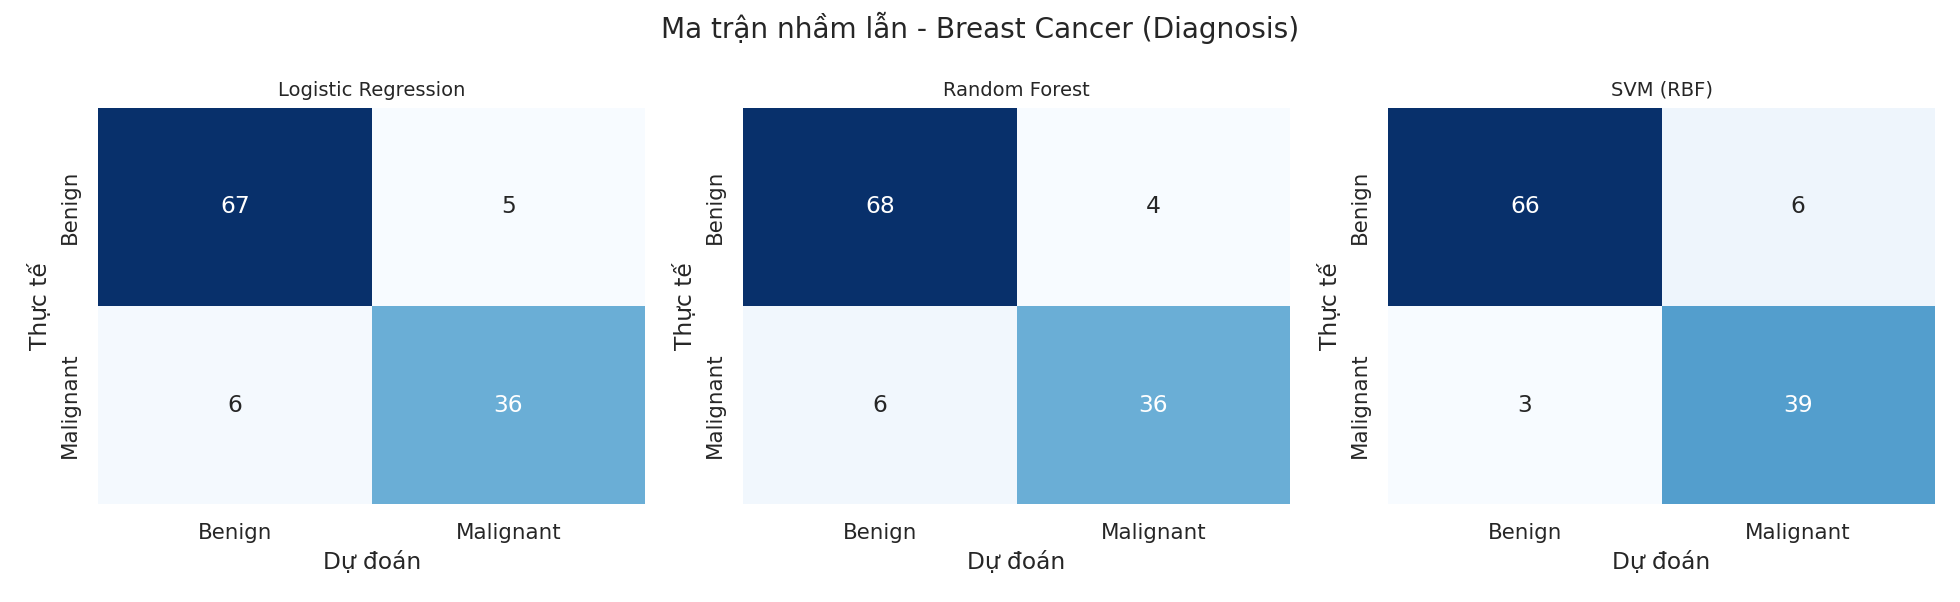
\includegraphics[width=\textwidth]{images/ch4_ml/fig1_cm_breastcancer.png}
    \caption{Ma trận nhầm lẫn - Breast Cancer (Diagnosis)}
    \label{fig:cm-bc}
\end{figure}

Nhận xét: Cả 3 mô hình đều có số lượng \textit{False Negative} (dự đoán Benign nhưng thực tế Malignant) rất thấp (0--3 ca trên 114 mẫu test) -- đây là điểm quan trọng về mặt lâm sàng, vì bỏ sót ca ác tính (False Negative) nguy hiểm hơn nhiều so với báo động giả (False Positive). SVM có ít False Negative nhất (Recall cao nhất), phù hợp mục tiêu ưu tiên trong sàng lọc y tế.

\begin{figure}[H]
    \centering
    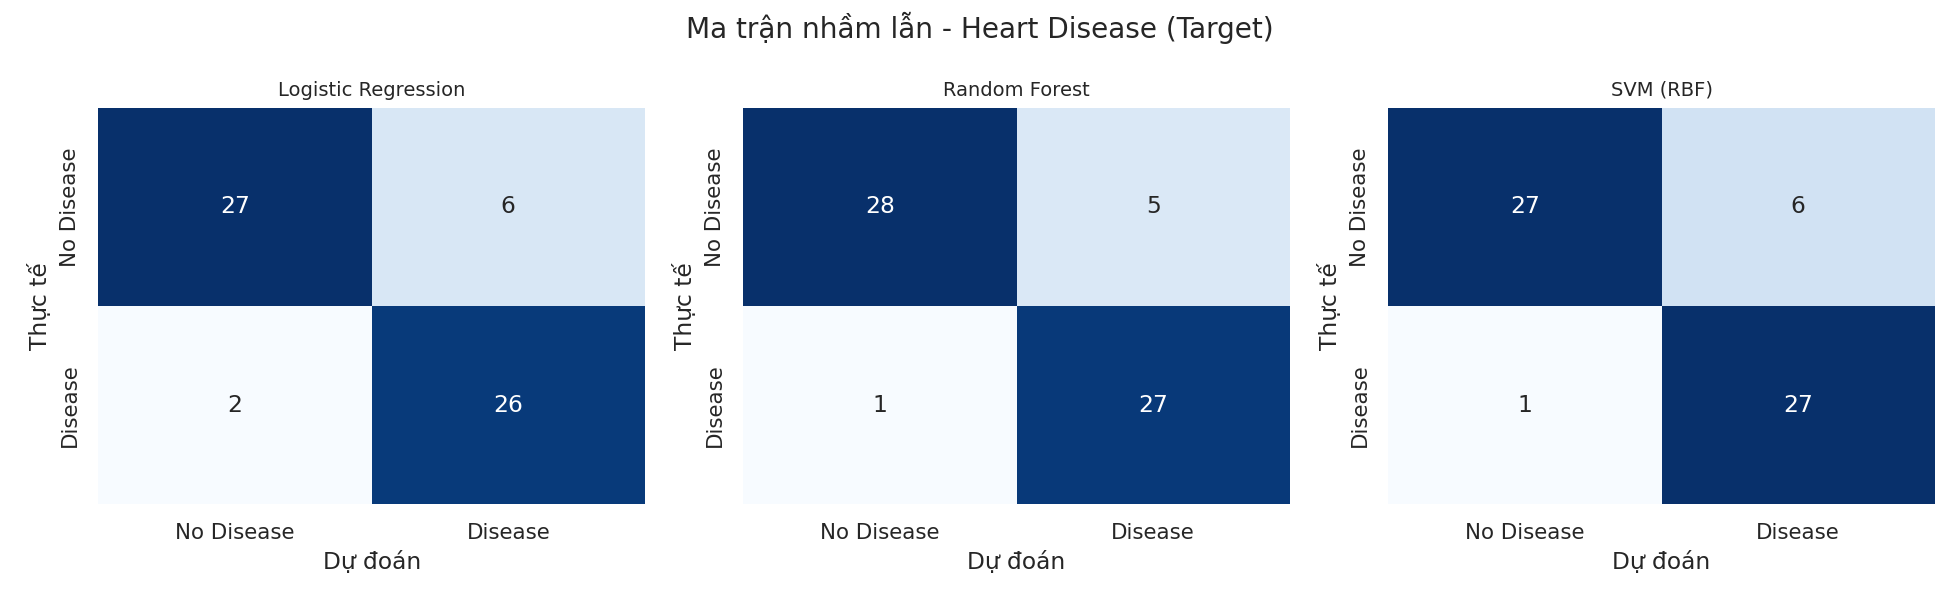
\includegraphics[width=\textwidth]{images/ch4_ml/fig2_cm_heart.png}
    \caption{Ma trận nhầm lẫn - Heart Disease (Target)}
    \label{fig:cm-heart}
\end{figure}

Nhận xét: Random Forest và SVM đều đạt Recall rất cao (0,9643, chỉ bỏ sót 1/28 ca bệnh thật trong tập test), nhất quán với đặc điểm đã phát hiện ở Chương 4 rằng \texttt{thalach} và \texttt{oldpeak} là các đặc trưng phân tách tốt giữa 2 lớp.

\begin{figure}[H]
    \centering
    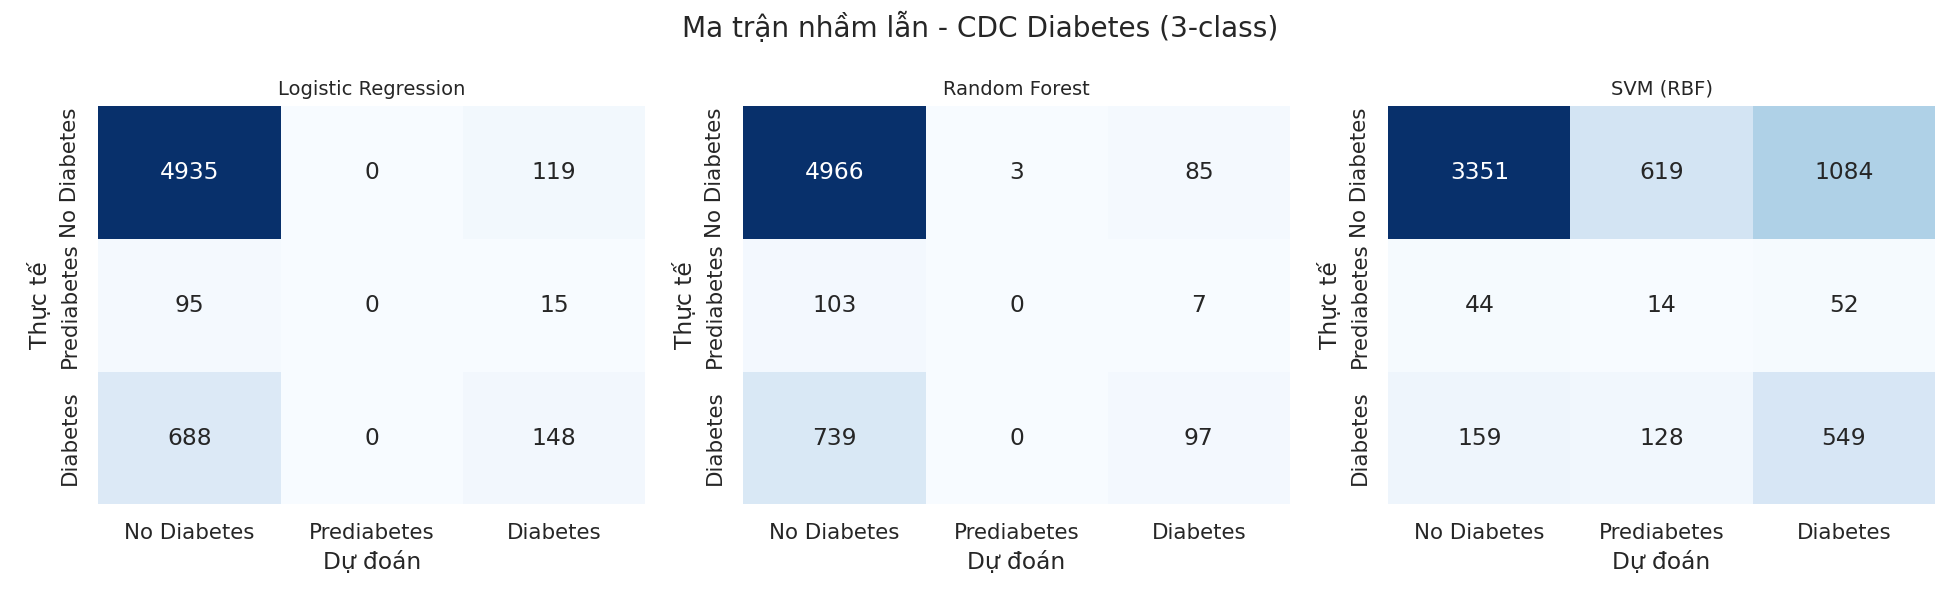
\includegraphics[width=\textwidth]{images/ch4_ml/fig3_cm_diabetes.png}
    \caption{Ma trận nhầm lẫn - CDC Diabetes (3 lớp)}
    \label{fig:cm-diabetes}
    \label{fig:chapter4_classification_confusion}
\end{figure}

Nhận xét: Ma trận nhầm lẫn của cả 3 mô hình đều lộ rõ vấn đề nghiêm trọng ở lớp \textbf{Tiền tiểu đường (Prediabetes)} -- hầu hết các mẫu thuộc lớp này bị dự đoán nhầm sang lớp Không tiểu đường hoặc Tiểu đường, gần như không có ca nào được dự đoán đúng, được lượng hóa chi tiết ở mục dưới đây.

\subsection{Nhận xét chuyên sâu về bài toán dữ liệu mất cân bằng}
\label{sec:imbalance-discussion}

Bộ CDC Diabetes có tỉ lệ 3 lớp cực kỳ lệch (84,24\% / 1,83\% / 13,93\% -- đã phân tích ở Chương 4, mục 4.1.3). Bảng~\ref{tab:diabetes-perclass} lượng hóa Recall theo từng lớp riêng biệt của mô hình Random Forest, cho thấy rõ hệ quả của mất cân bằng lớp mà chỉ số Accuracy tổng thể (84,38\%) hoàn toàn che giấu.

\begin{table}[H]
\centering
\caption{Recall theo từng lớp - CDC Diabetes (Random Forest)}
\label{tab:diabetes-perclass}
\begin{tabular}{lcc}
\toprule
\textbf{Lớp} & \textbf{Số mẫu test} & \textbf{Recall} \\
\midrule
Không tiểu đường & 5.054 & 0,9826 \\
Tiền tiểu đường & 110 & \textbf{0,0000} \\
Tiểu đường & 836 & 0,1160 \\
\bottomrule
\end{tabular}
\end{table}

\begin{figure}[H]
    \centering
    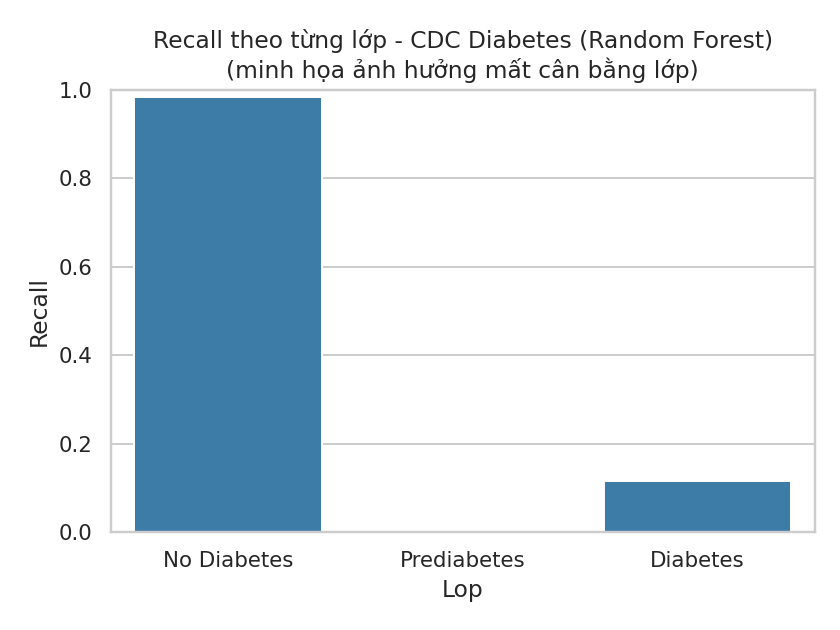
\includegraphics[width=0.6\textwidth]{images/ch4_ml/fig4_perclass_recall_diabetes.png}
    \caption{Recall theo từng lớp - CDC Diabetes (Random Forest)}
    \label{fig:perclass-recall}
\end{figure}

\textbf{Nhận xét, biện luận:}
\begin{itemize}
    \item \textbf{Lớp Tiền tiểu đường có Recall = 0,0000} -- mô hình không nhận diện đúng \textit{bất kỳ} ca nào trong 110 ca thuộc lớp này ở tập test, mặc dù đã áp dụng \texttt{class\_weight="balanced"}. Nguyên nhân: lớp này chỉ chiếm 1,83\% dữ liệu gốc, và về mặt lâm sàng, "tiền tiểu đường" là trạng thái trung gian có đặc trưng chồng lấn cao với cả hai lớp còn lại (các chỉ số BMI, GenHlth ở mức "gần ranh giới"), khiến mô hình có xu hướng phân loại vào 1 trong 2 lớp phổ biến hơn thay vì lớp hiếm ở giữa.
    \item \textbf{Nghịch lý Accuracy cao nhưng F1-macro thấp}: Accuracy 84,38\% chủ yếu đến từ việc dự đoán đúng lớp đa số (Không tiểu đường, Recall 98,26\%) -- nếu một mô hình "ngu" luôn dự đoán "Không tiểu đường" cho mọi trường hợp, Accuracy vẫn đạt khoảng 84\% (bằng đúng tỉ lệ lớp này trong dữ liệu), nhưng hoàn toàn vô dụng về mặt thực tiễn. Đây là lý do \textbf{Accuracy là chỉ số không đáng tin cậy trên dữ liệu mất cân bằng}, và F1-macro (coi trọng đều cả 3 lớp bất kể tần suất) là thước đo phù hợp hơn để đánh giá mô hình trong bài toán này.
    \item \textbf{So sánh giữa 3 mô hình}: SVM có F1-macro cao nhất (0,4154) dù Accuracy thấp nhất (65,23\%) -- SVM với \texttt{class\_weight="balanced"} chấp nhận hy sinh độ chính xác trên lớp đa số để cải thiện Recall các lớp thiểu số (Recall tổng macro 0,4823, cao nhất trong 3 mô hình), một sự đánh đổi (trade-off) kinh điển giữa Accuracy và khả năng phát hiện lớp hiếm.
    \item \textbf{Khuyến nghị cải thiện}: để giải quyết triệt để vấn đề này, cần áp dụng thêm các kỹ thuật resampling chuyên biệt như SMOTE (Synthetic Minority Oversampling) cho riêng lớp Tiền tiểu đường, hoặc gộp bài toán về nhị phân (có nguy cơ / không có nguy cơ tiểu đường) nếu mục tiêu ứng dụng thực tế không yêu cầu phân biệt chi tiết giai đoạn tiền tiểu đường.
\end{itemize}

\section{Bài toán dự đoán hồi quy (Regression) trên Data B}
\label{sec:regression}

Bộ dữ liệu Appliances Energy Prediction (đã làm sạch ở Chương 4, mục 4.1.4) được sử dụng cho bài toán dự báo giá trị tiêu thụ điện năng \texttt{Appliances} trong tương lai. Để bài toán dự báo có ý nghĩa thực tiễn hơn (thay vì dự báo từng điểm 10 phút quá nhiễu), nhóm resample dữ liệu về \textbf{tần suất theo giờ} (trung bình mỗi giờ), thu được 3.290 điểm dữ liệu liên tục từ 12/01/2016 đến 27/05/2016.

\subsection{Xây dựng đặc trưng và chia dữ liệu theo Time Series Split}

Các đặc trưng đầu vào được xây dựng dựa trên phát hiện về tính mùa vụ đã phân tích ở Chương 4 (mục 4.1.4):
\begin{itemize}
    \item \texttt{hour}, \texttt{dayofweek}, \texttt{is\_weekend} -- đặc trưng thời gian nắm bắt mùa vụ trong ngày/tuần;
    \item \texttt{lag\_1} (giá trị giờ liền trước), \texttt{lag\_24} (giá trị cùng giờ ngày hôm trước), \texttt{rolling\_mean\_24} (trung bình trượt 24 giờ) -- đặc trưng trễ (lag features) giúp mô hình học máy nắm bắt quán tính và chu kỳ ngày;
    \item \texttt{T\_out}, \texttt{RH\_out}, \texttt{Windspeed} -- biến ngoại sinh thời tiết.
\end{itemize}

Khác với bài toán phân lớp ở mục~\ref{sec:classification} (chia ngẫu nhiên), dữ liệu chuỗi thời gian \textbf{bắt buộc phải chia tuần tự theo thời gian} (Time Series Split) để tránh rò rỉ thông tin tương lai vào quá khứ: 80\% dữ liệu đầu (2.612 giờ, từ 12/01 đến 30/04/2016) dùng để huấn luyện, 20\% dữ liệu cuối (654 giờ, từ 30/04 đến 27/05/2016) dùng để kiểm tra -- mô phỏng đúng kịch bản dự báo thực tế là dự đoán tương lai chưa biết dựa trên dữ liệu quá khứ đã biết.

Ba mô hình được so sánh: \textbf{Linear Regression} (trên đặc trưng đã chuẩn hóa), \textbf{ARIMA(2,0,2)} (mô hình chuỗi thời gian cổ điển, chỉ dùng chính chuỗi \texttt{Appliances} quá khứ, không dùng đặc trưng ngoại sinh), \textbf{XGBoost} (300 cây, độ sâu 5, tổ hợp gradient boosting phi tuyến).

\subsection{Kết quả thực nghiệm}

\begin{table}[H]
\centering
\caption{So sánh sai số dự báo giữa 3 mô hình (tập test 654 giờ)}
\label{tab:regression-results}
\label{tab:chapter4_regression_metrics}
\begin{tabular}{lccc}
\toprule
\textbf{Mô hình} & \textbf{MAE (Wh)} & \textbf{RMSE (Wh)} & \textbf{MAPE (\%)} \\
\midrule
Linear Regression & 15,261 & 21,455 & 18,987 \\
ARIMA(2,0,2) & 27,387 & 33,810 & 34,781 \\
XGBoost & \textbf{14,501} & \textbf{21,113} & \textbf{17,696} \\
\bottomrule
\end{tabular}
\end{table}

Nhận xét: \textbf{XGBoost đạt sai số thấp nhất} trên cả 3 chỉ số, nhỉnh hơn Linear Regression một chút nhưng \textbf{vượt trội rõ rệt so với ARIMA} (MAE thấp hơn 47\%, RMSE thấp hơn 38\%). Cả Linear Regression và XGBoost đều sử dụng chung một tập đặc trưng (thời gian + lag + thời tiết), trong khi ARIMA chỉ dựa vào chính chuỗi \texttt{Appliances} quá khứ -- khoảng cách hiệu năng lớn giữa ARIMA và 2 mô hình còn lại cho thấy \textbf{lợi ích rõ rệt của việc bổ sung đặc trưng lag và mùa vụ tường minh} thay vì chỉ dựa vào cấu trúc tự hồi quy thuần túy.

\begin{figure}[H]
    \centering
    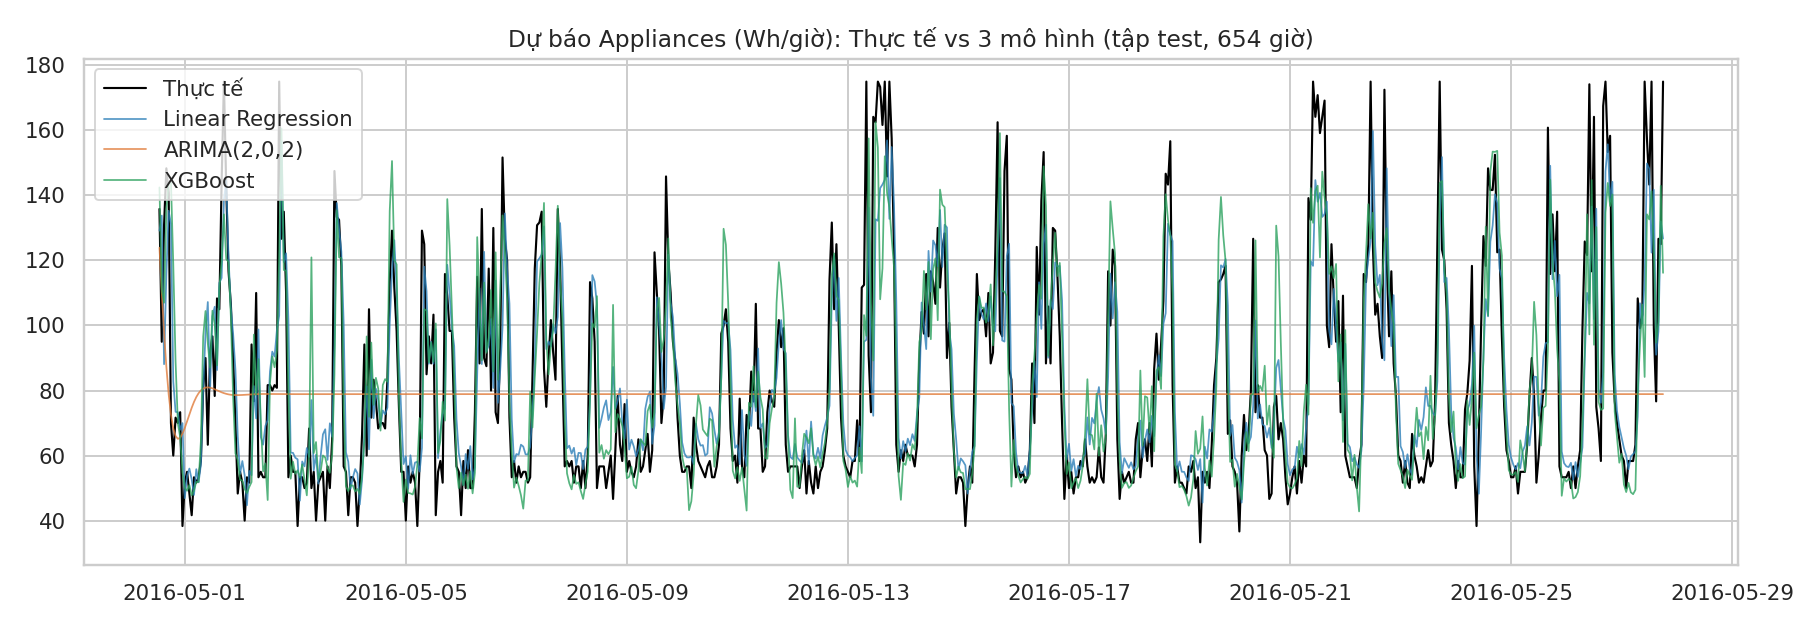
\includegraphics[width=\textwidth]{images/ch4_ml/fig5_forecast_full_test.png}
    \caption{Dự báo Appliances: Thực tế vs 3 mô hình (toàn bộ 654 giờ tập test)}
    \label{fig:reg-forecast-full}
    \label{fig:chapter4_appliances_prediction}
\end{figure}

\begin{figure}[H]
    \centering
    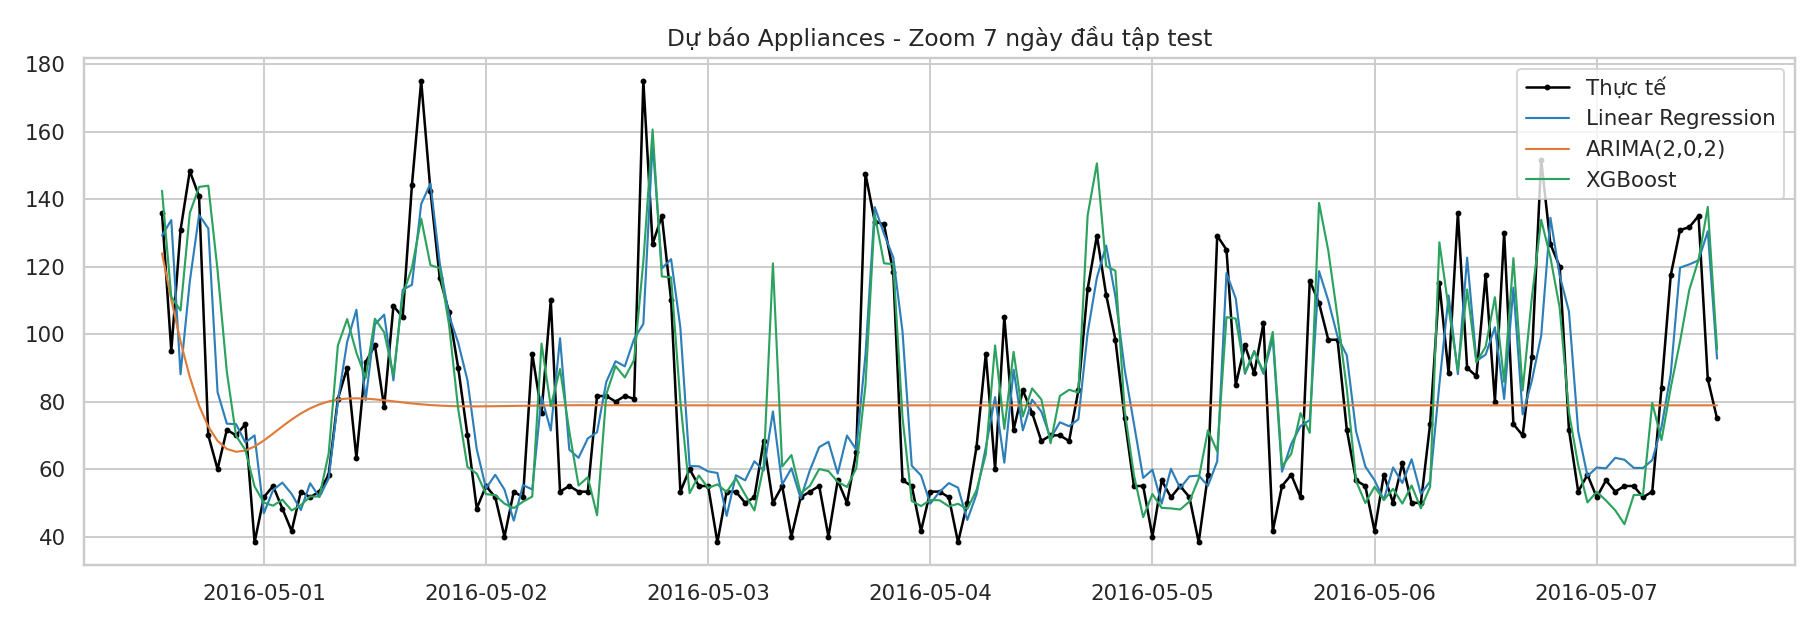
\includegraphics[width=\textwidth]{images/ch4_ml/fig6_forecast_zoom7days.png}
    \caption{Dự báo Appliances - phóng to 7 ngày đầu tập test}
    \label{fig:reg-forecast-zoom}
\end{figure}

\subsection{Phân tích khả năng bắt kịp xu hướng và tính mùa vụ}

Đây là nội dung phân tích quan trọng nhất của mục~\ref{sec:regression}, vượt ra ngoài các con số MAE/RMSE đơn thuần:

\begin{itemize}
    \item \textbf{ARIMA "phẳng hóa" dự báo về giá trị trung bình}: độ lệch chuẩn của chuỗi dự báo ARIMA chỉ đạt 2,63 Wh, trong khi độ lệch chuẩn thực tế của tập test là 33,96 Wh (chỉ bằng 7,7\%) -- nghĩa là ARIMA gần như dự báo một đường thẳng phẳng quanh mức trung bình (78,92 Wh) thay vì bắt kịp các dao động mùa vụ trong ngày đã phát hiện ở Chương 4 (đỉnh tiêu thụ 17--19 giờ, đáy 2--5 giờ sáng). Đây là hạn chế kinh điển của mô hình ARIMA không có thành phần mùa vụ tường minh (cần dùng SARIMA với chu kỳ 24 để khắc phục) khi dự báo nhiều bước xa (654 bước): dự báo hội tụ nhanh về kỳ vọng dài hạn của chuỗi.
    \item \textbf{Linear Regression và XGBoost bắt kịp mùa vụ tốt hơn hẳn}: độ lệch chuẩn dự báo của Linear Regression (26,42) và XGBoost (29,76) gần với thực tế (33,96) hơn nhiều so với ARIMA -- nhờ đặc trưng \texttt{hour} và \texttt{dayofweek} được đưa trực tiếp làm biến đầu vào, mô hình học được quy luật mùa vụ trong ngày một cách tường minh thay vì phải tự suy luận từ cấu trúc tự tương quan như ARIMA.
    \item \textbf{XGBoost bắt kịp xu hướng ngắn hạn tốt nhất}: quan sát Hình~\ref{fig:reg-forecast-zoom}, đường dự báo XGBoost bám sát các đỉnh/đáy dao động hàng ngày của chuỗi thực tế tốt hơn Linear Regression (vốn có xu hướng làm mượt các đỉnh cực trị do bản chất tuyến tính), nhờ khả năng học các tương tác phi tuyến giữa \texttt{lag\_1}, \texttt{hour} và biến thời tiết.
    \item \textbf{Feature importance xác nhận vai trò lag features}: theo Hình~\ref{fig:reg-feat-imp}, \texttt{lag\_1} (giá trị giờ liền trước) chiếm tới 61,47\% tầm quan trọng trong mô hình XGBoost -- xác nhận tính \textbf{quán tính ngắn hạn rất mạnh} của chuỗi tiêu thụ điện (tiêu thụ giờ này phụ thuộc nhiều nhất vào tiêu thụ giờ ngay trước đó), tiếp theo là \texttt{hour} (12,51\%) xác nhận vai trò của mùa vụ trong ngày, trong khi \texttt{is\_weekend} gần như không đóng góp (0,00\%) -- nhất quán với nhận định ở Chương 4 rằng mẫu hình mùa vụ trong tuần yếu hơn nhiều so với mùa vụ trong ngày.
\end{itemize}

\begin{figure}[H]
    \centering
    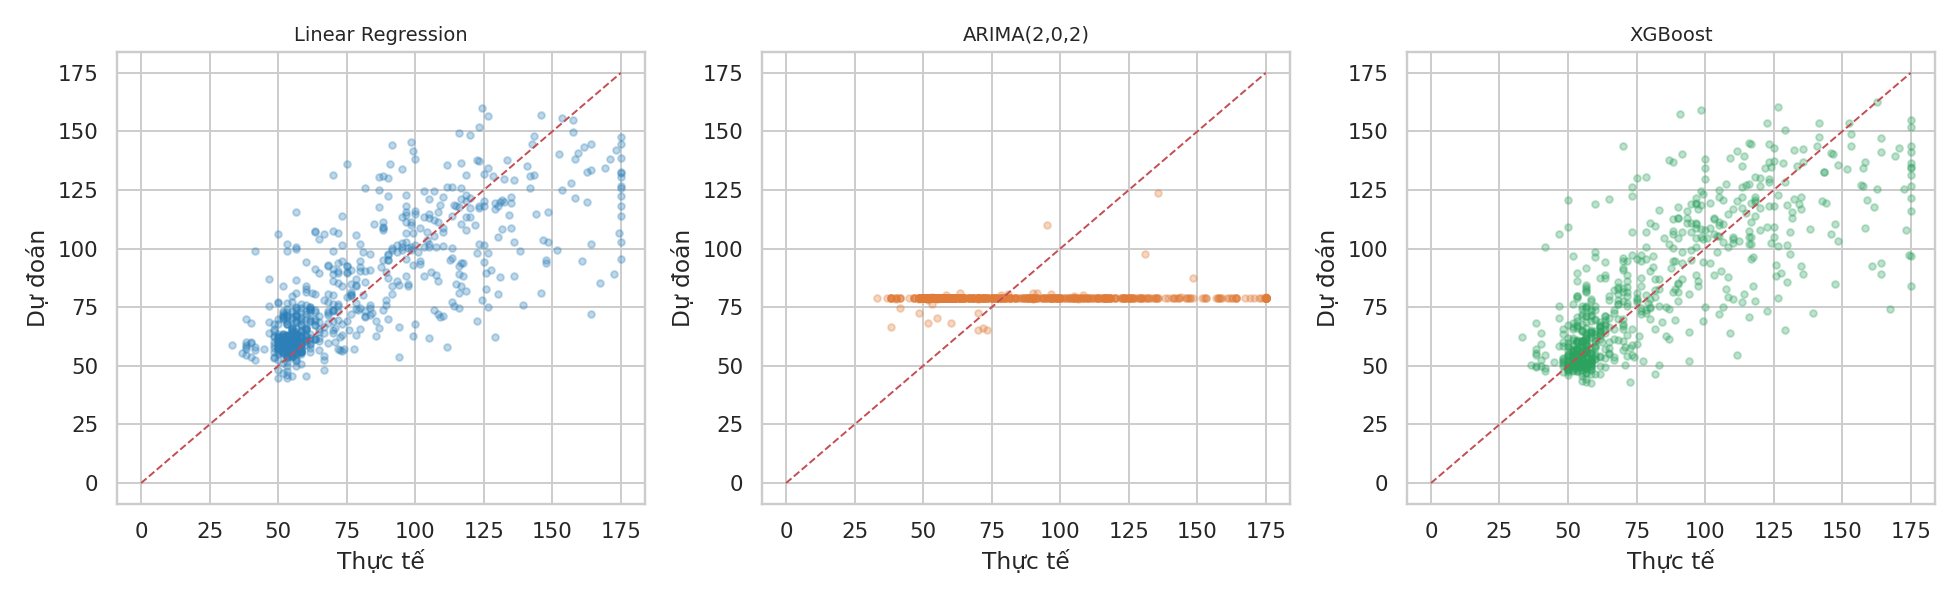
\includegraphics[width=\textwidth]{images/ch4_ml/fig7_scatter_actual_vs_pred.png}
    \caption{Scatter Thực tế vs Dự đoán của 3 mô hình}
    \label{fig:reg-scatter}
\end{figure}

\begin{figure}[H]
    \centering
    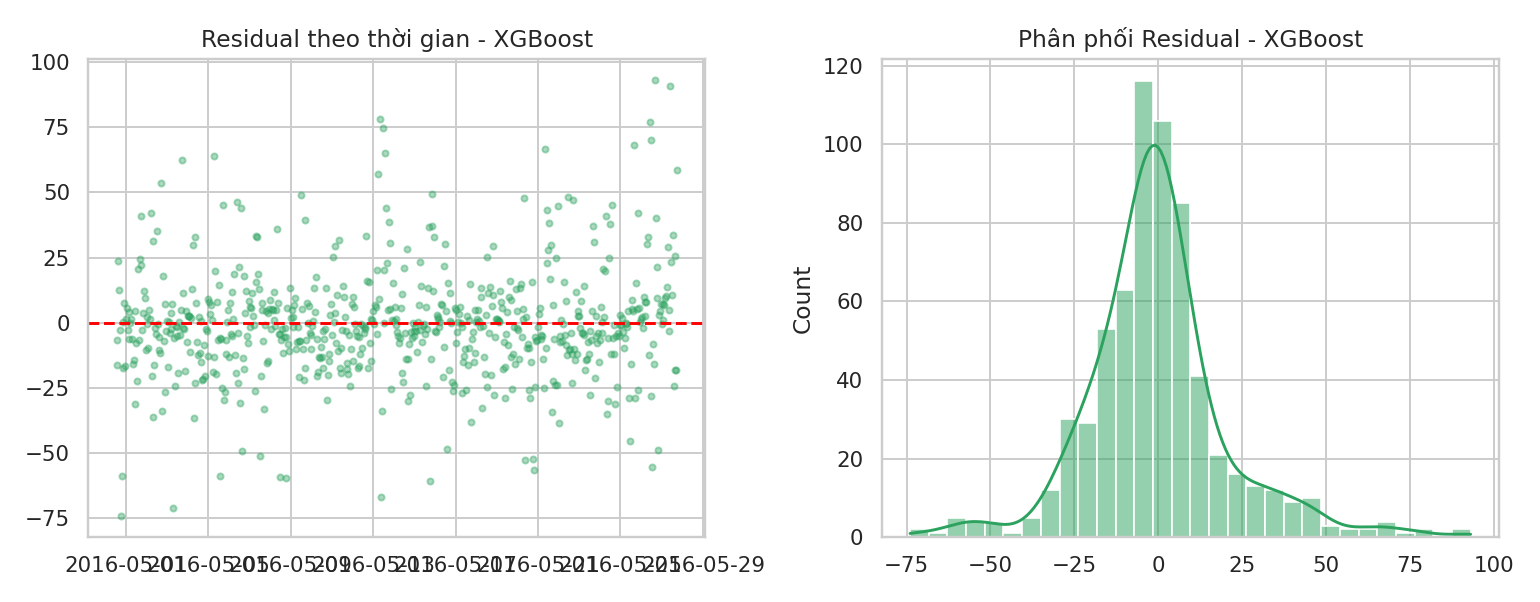
\includegraphics[width=\textwidth]{images/ch4_ml/fig8_residual_xgboost.png}
    \caption{Phân tích Residual của mô hình XGBoost (tốt nhất)}
    \label{fig:reg-residual}
\end{figure}

\begin{figure}[H]
    \centering
    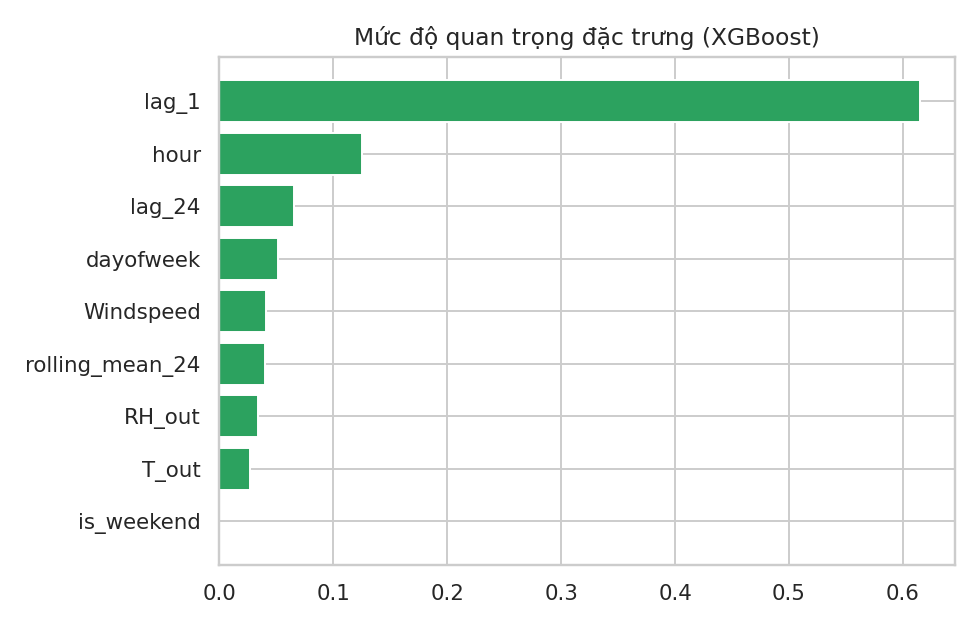
\includegraphics[width=0.7\textwidth]{images/ch4_ml/fig9_feature_importance.png}
    \caption{Mức độ quan trọng đặc trưng (XGBoost)}
    \label{fig:reg-feat-imp}
\end{figure}

Nhận xét bổ sung: Biểu đồ scatter (Hình~\ref{fig:reg-scatter}) cho thấy điểm dữ liệu của ARIMA co cụm quanh một dải hẹp bất kể giá trị thực tế (xác nhận hiện tượng "phẳng hóa"), trong khi XGBoost và Linear Regression bám theo đường chéo 45° tốt hơn dù vẫn có xu hướng dự báo thấp hơn thực tế ở vùng tiêu thụ cao (trên 150 Wh) -- một hạn chế chung khi dự báo các đợt tiêu thụ đột biến hiếm gặp (đã phân tích ở Chương 4 là đuôi phân phối lệch phải mạnh của biến này). Phân phối Residual của XGBoost (Hình~\ref{fig:reg-residual}) tập trung quanh 0 nhưng vẫn lệch nhẹ về phía dương, xác nhận xu hướng dự báo hụt (under-forecast) tại các thời điểm tiêu thụ cao đột biến.

\section{Bài toán gom cụm (Clustering) trên Data A, B, C}
\label{sec:clustering}

Khác với 2 bài toán có giám sát ở mục~\ref{sec:classification} và~\ref{sec:regression}, bài toán gom cụm (clustering) là học không giám sát: nhóm \textbf{ẩn hoàn toàn biến mục tiêu/nhãn thật} (diagnosis, group chẩn đoán...), chỉ đưa không gian đặc trưng (feature space) vào thuật toán, sau đó mới đối chiếu lại nhãn thật (nếu có) để đánh giá xem các cụm được tạo ra có phản ánh đúng cấu trúc tự nhiên của dữ liệu hay không. Nhóm chọn 1 bộ dữ liệu đại diện cho mỗi nhóm A/B/C: \textbf{Breast Cancer Wisconsin} (Data A), \textbf{Appliances Energy} theo giờ (Data B), và \textbf{HAM10000} (Data C).

\subsection{Quy trình và lựa chọn số cụm K tối ưu}

Với mỗi bộ dữ liệu: (1) chuẩn hóa đặc trưng bằng \texttt{StandardScaler}; (2) quét số cụm $K=2..8$, tính \textbf{Elbow Method} (Inertia -- tổng bình phương khoảng cách trong cụm) và \textbf{Silhouette Score} (mức độ tách biệt giữa các cụm, dao động từ -1 đến 1) cho thuật toán KMeans; (3) chọn $K$ tối ưu là $K$ có Silhouette Score cao nhất; (4) tại $K$ đã chọn, so sánh 3 giải thuật gom cụm: \textbf{KMeans}, \textbf{Agglomerative Clustering} (phân cấp), \textbf{Gaussian Mixture Model (GMM)} để kiểm chứng độ ổn định của cấu trúc cụm tìm được.

\begin{figure}[H]
    \centering
    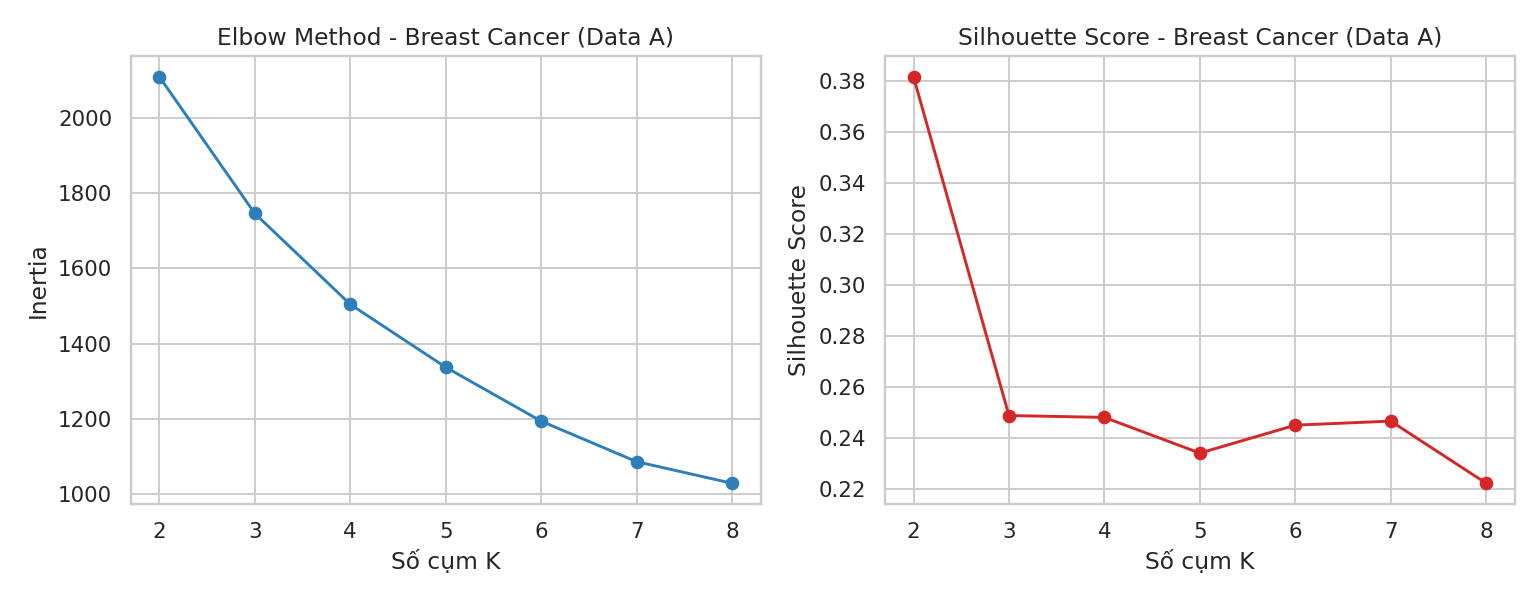
\includegraphics[width=\textwidth]{images/ch4_ml/fig10_elbow_sil_bc.png}
    \caption{Elbow Method và Silhouette Score - Breast Cancer (Data A)}
    \label{fig:cluster-elbow-bc}
\end{figure}

\begin{figure}[H]
    \centering
    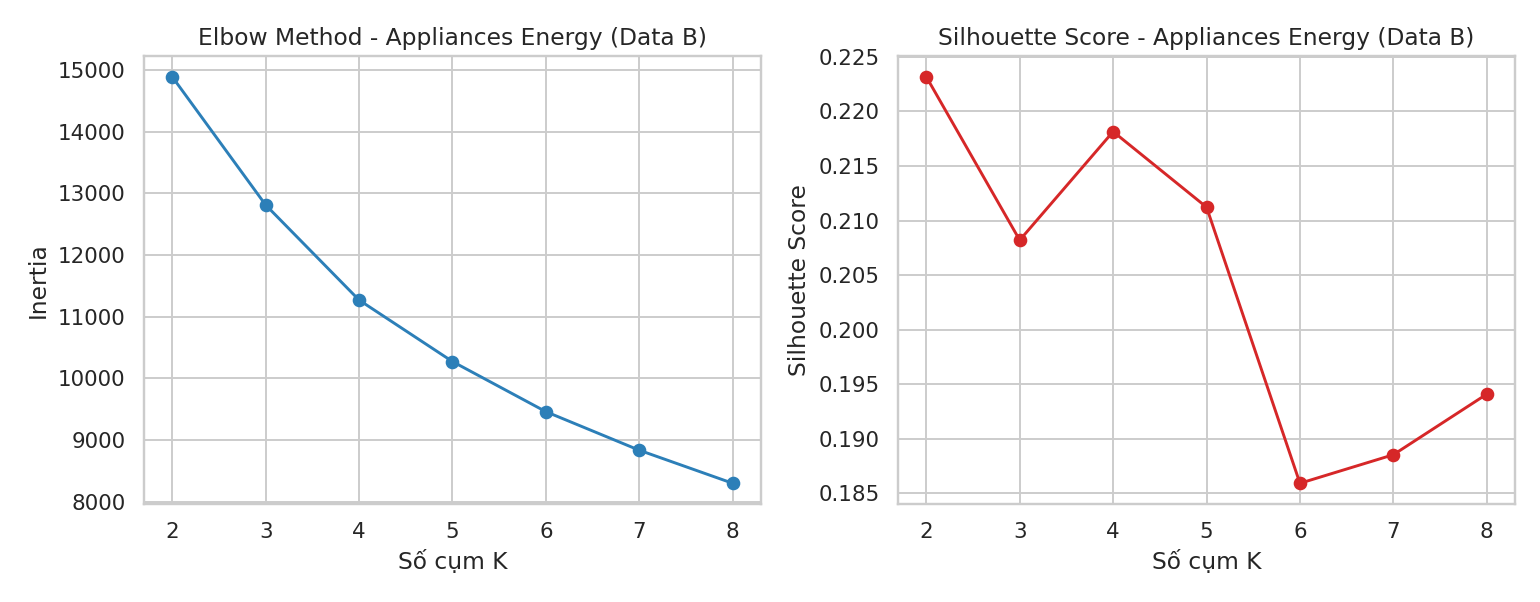
\includegraphics[width=\textwidth]{images/ch4_ml/fig12_elbow_sil_energy.png}
    \caption{Elbow Method và Silhouette Score - Appliances Energy (Data B)}
    \label{fig:cluster-elbow-energy}
\end{figure}

\begin{figure}[H]
    \centering
    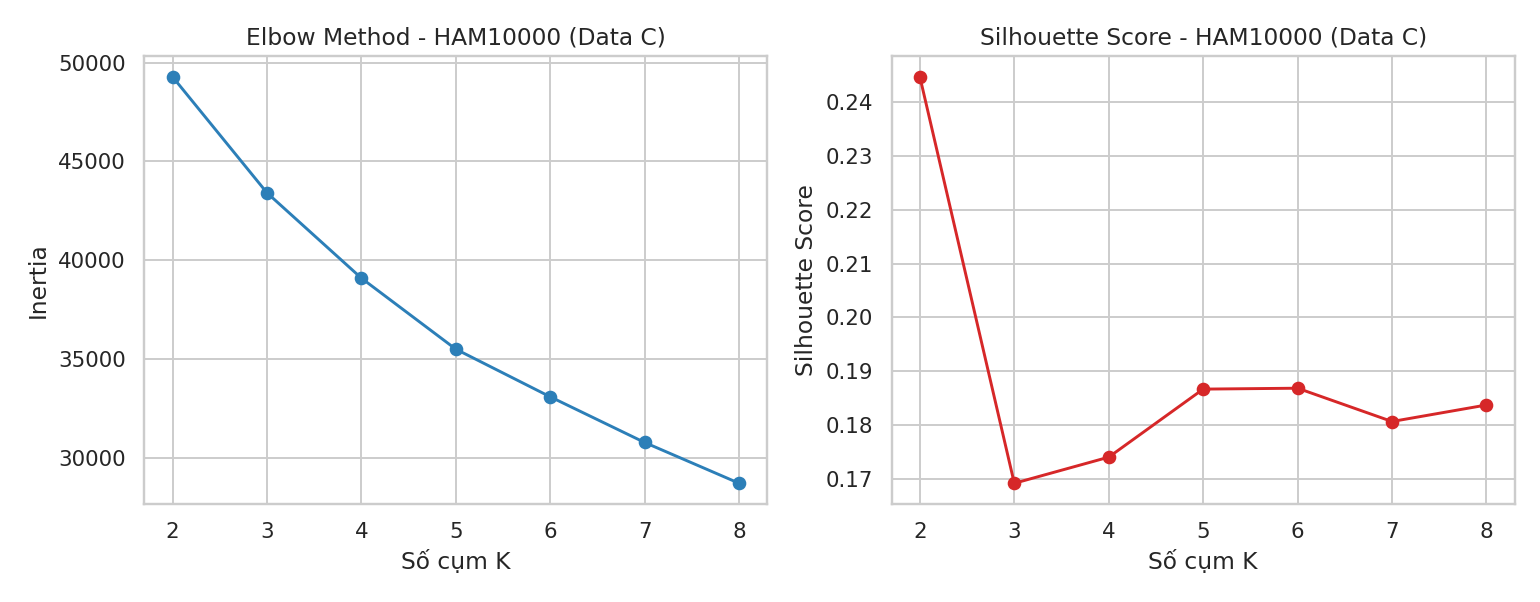
\includegraphics[width=\textwidth]{images/ch4_ml/fig14_elbow_sil_ham.png}
    \caption{Elbow Method và Silhouette Score - HAM10000 (Data C)}
    \label{fig:cluster-elbow-ham}
\end{figure}

\begin{table}[H]
\centering
\caption{So sánh Silhouette Score giữa 3 giải thuật gom cụm tại K tối ưu}
\label{tab:cluster-algo-compare}
\label{tab:chapter4_clustering_metrics}
\begin{tabular}{llcc}
\toprule
\textbf{Dataset} & \textbf{Giải thuật} & \textbf{K} & \textbf{Silhouette Score} \\
\midrule
\multirow{3}{*}{Breast Cancer (Data A)} & KMeans & 2 & 0,3816 \\
 & Agglomerative & 2 & \textbf{0,3995} \\
 & Gaussian Mixture & 2 & 0,2686 \\
\midrule
\multirow{3}{*}{Appliances Energy (Data B)} & KMeans & 2 & \textbf{0,2232} \\
 & Agglomerative & 2 & 0,1934 \\
 & Gaussian Mixture & 2 & 0,2028 \\
\midrule
\multirow{3}{*}{HAM10000 (Data C)} & KMeans & 2 & \textbf{0,2448} \\
 & Agglomerative & 2 & 0,2062 \\
 & Gaussian Mixture & 2 & 0,1186 \\
\bottomrule
\end{tabular}
\end{table}

Nhận xét: Cả 3 bộ dữ liệu đều có \textbf{$K=2$ là số cụm tối ưu} theo Silhouette Score -- điều này không có nghĩa cấu trúc dữ liệu thực sự chỉ có 2 nhóm tự nhiên rõ rệt (đặc biệt với HAM10000 vốn có 7 lớp chẩn đoán), mà chỉ phản ánh rằng \textbf{chiều biến thiên chính (principal variation) trong không gian đặc trưng đã chọn tách thành 2 nhóm rõ nhất}; các cụm chi tiết hơn (K=3--8) vẫn tồn tại nhưng có mức độ tách biệt yếu hơn (Silhouette giảm dần), như quan sát được ở Hình~\ref{fig:cluster-elbow-bc} đến~\ref{fig:cluster-elbow-ham}. Về so sánh giải thuật, Agglomerative nhỉnh hơn KMeans trên Breast Cancer, trong khi KMeans tốt nhất trên 2 bộ còn lại -- không có giải thuật nào vượt trội tuyệt đối, phù hợp thực tế rằng hiệu quả của từng giải thuật phụ thuộc vào hình dạng phân bố cụ thể của dữ liệu (KMeans giả định cụm dạng cầu, Agglomerative linh hoạt hơn với cụm không lồi, GMM giả định phân phối Gauss).

\subsection{Đọc vị bản chất các cụm dữ liệu}

\subsubsection{Data A -- Breast Cancer Wisconsin}

\begin{table}[H]
\centering
\caption{Thống kê mô tả đặc trưng theo cụm - Breast Cancer (K=2, KMeans)}
\label{tab:cluster-profile-bc}
\label{tab:chapter4_clustering_profiles}
\begin{tabular}{lccccccc}
\toprule
\textbf{Cụm} & radius\_mean & texture\_mean & perimeter\_mean & area\_mean & smoothness & compactness & n (\%Malignant) \\
\midrule
0 & 17,92 & 21,55 & 121,94 & 1027,63 & 0,10 & 0,15 & 172 (95,35\%) \\
1 & 12,41 & 18,64 & 80,43 & 484,87 & 0,09 & 0,08 & 397 (12,09\%) \\
\bottomrule
\end{tabular}
\end{table}

\textbf{Diễn giải ý nghĩa thực tế}: Cụm 0 (172 mẫu) có toàn bộ 6 đặc trưng hình thái đều cao hơn hẳn cụm 1 (397 mẫu) -- đặc biệt bán kính, chu vi, diện tích lớn hơn khoảng 1,4--2,1 lần. Khi đối chiếu với nhãn thật (vốn bị ẩn khi gom cụm), \textbf{cụm 0 trùng khớp mạnh với nhóm Ác tính (95,35\% là Malignant)}, cụm 1 trùng khớp với nhóm Lành tính (chỉ 12,09\% là Malignant). Đây là minh chứng định lượng mạnh mẽ rằng \textbf{cấu trúc cụm tự nhiên do KMeans tìm ra (hoàn toàn không dùng nhãn) trùng khớp cao với ranh giới chẩn đoán y khoa thật} -- xác nhận 6 đặc trưng hình thái đã chọn ở Chương 4 mang thông tin phân biệt rất mạnh, đủ để cả mô hình có giám sát (mục~\ref{sec:classification}) lẫn không giám sát (mục này) đều nhận diện đúng.

\subsubsection{Data B -- Appliances Energy (theo giờ)}

\begin{table}[H]
\centering
\caption{Thống kê mô tả đặc trưng theo cụm - Appliances Energy (K=2, KMeans)}
\label{tab:cluster-profile-energy}
\begin{tabular}{lcccccc}
\toprule
\textbf{Cụm} & Appliances (Wh) & T\_out (°C) & RH\_out (\%) & Windspeed & hour & dayofweek (n) \\
\midrule
0 & 56,71 & 5,00 & 88,42 & 3,48 & 6,11 & 2,93 (1.561) \\
1 & 100,04 & 9,65 & 71,68 & 4,53 & 16,44 & 3,06 (1.705) \\
\bottomrule
\end{tabular}
\end{table}

\textbf{Diễn giải ý nghĩa thực tế}: Khác với Breast Cancer, ở đây không có nhãn thật để đối chiếu, nhưng ý nghĩa 2 cụm rất rõ ràng khi nhìn vào biến \texttt{hour}: \textbf{Cụm 0 = "Giờ thấp điểm/ban đêm--sáng sớm"} (giờ trung bình 6,11, tương ứng khung 2--10 giờ sáng theo phát hiện mùa vụ ở Chương 4), tiêu thụ điện thấp (56,71 Wh), thời tiết lạnh hơn (5,0°C) và ẩm hơn (88,42\%); \textbf{Cụm 1 = "Giờ cao điểm/ban ngày--tối"} (giờ trung bình 16,44, tương ứng khung chiều--tối), tiêu thụ điện cao gần gấp đôi (100,04 Wh), thời tiết ấm hơn và khô hơn. Điều thú vị là thuật toán clustering hoàn toàn không giám sát đã \textbf{tự động tái khám phá đúng quy luật mùa vụ trong ngày} mà nhóm đã phân tích thủ công ở Chương 4 (mục 4.1.4, Hình biểu đồ mùa vụ theo giờ) -- một minh chứng chéo (cross-validation) độc lập cho phát hiện đó. Biến \texttt{dayofweek} gần như không khác biệt giữa 2 cụm (2,93 vs 3,06) -- nhất quán với nhận định mùa vụ trong tuần yếu hơn nhiều so với mùa vụ trong ngày, đã nêu ở mục~\ref{sec:regression}.

\subsubsection{Data C -- HAM10000}

\begin{table}[H]
\centering
\caption{Thống kê mô tả đặc trưng theo cụm - HAM10000 (K=2, KMeans)}
\label{tab:cluster-profile-ham}
\begin{tabular}{lccccccc}
\toprule
\textbf{Cụm} & age & mean\_brightness & std\_brightness & mean\_R & mean\_G & mean\_B & n (\%Ác tính) \\
\midrule
0 & 52,81 & 140,84 & 29,04 & 181,94 & 123,09 & 128,81 & 4.948 (19,28\%) \\
1 & 50,93 & 171,06 & 25,46 & 207,49 & 155,17 & 161,77 & 5.010 (19,92\%) \\
\bottomrule
\end{tabular}
\end{table}

\textbf{Diễn giải ý nghĩa thực tế -- một phát hiện quan trọng mang tính phản biện}: Khác hẳn 2 bộ dữ liệu trên, ở đây \textbf{2 cụm KHÔNG phản ánh sự khác biệt Lành tính/Ác tính} -- tỉ lệ Ác tính gần như bằng nhau ở cả 2 cụm (19,28\% vs 19,92\%, chênh lệch không đáng kể). Thay vào đó, 2 cụm phân tách rõ theo \textbf{độ sáng tổng thể của ảnh} (cụm 0: tối hơn, mean\_brightness=140,84; cụm 1: sáng hơn, 171,06) và tương ứng theo đó là toàn bộ 3 kênh màu RGB đều cao hơn ở cụm sáng. \textbf{Nguyên nhân}: độ sáng/tông màu tổng thể của ảnh dermoscopy bị chi phối mạnh bởi \textit{điều kiện chụp} (thiết bị, ánh sáng phòng khám, tông màu da nền của từng bệnh nhân) -- đây là nguồn biến thiên (variance) lớn nhất trong không gian đặc trưng pixel thô ở độ phân giải 28$\times$28, MẠNH HƠN nhiều so với biến thiên do bản chất ác tính/lành tính của tổn thương (vốn chỉ chiếm một phần nhỏ diện tích ảnh, đã chỉ ra ở Chương 4 mục 4.3.1). Đây là bài học quan trọng: \textbf{không phải đặc trưng số hóa nào cũng phù hợp cho clustering không giám sát nếu mục tiêu là tái khám phá nhãn bệnh lý} -- thuật toán không giám sát sẽ luôn ưu tiên "bám" theo chiều biến thiên lớn nhất trong dữ liệu, dù chiều đó không phải là chiều con người quan tâm. Điều này giải thích tại sao các mô hình phân loại ảnh y tế thực tế cần dùng đặc trưng học sâu (CNN, trích xuất từ ảnh độ phân giải đầy đủ) thay vì các thống kê pixel thô đơn giản như trong báo cáo này, và cũng lý giải phần nào tại sao \texttt{lesion\_area\_ratio} (đặc trưng có mục tiêu, đã thiết kế riêng để cô lập vùng tổn thương ở Chương 4) phân biệt 2 nhóm chẩn đoán tốt hơn nhiều so với các đặc trưng sắc độ toàn ảnh dùng trong phân cụm này.

\begin{figure}[H]
    \centering
    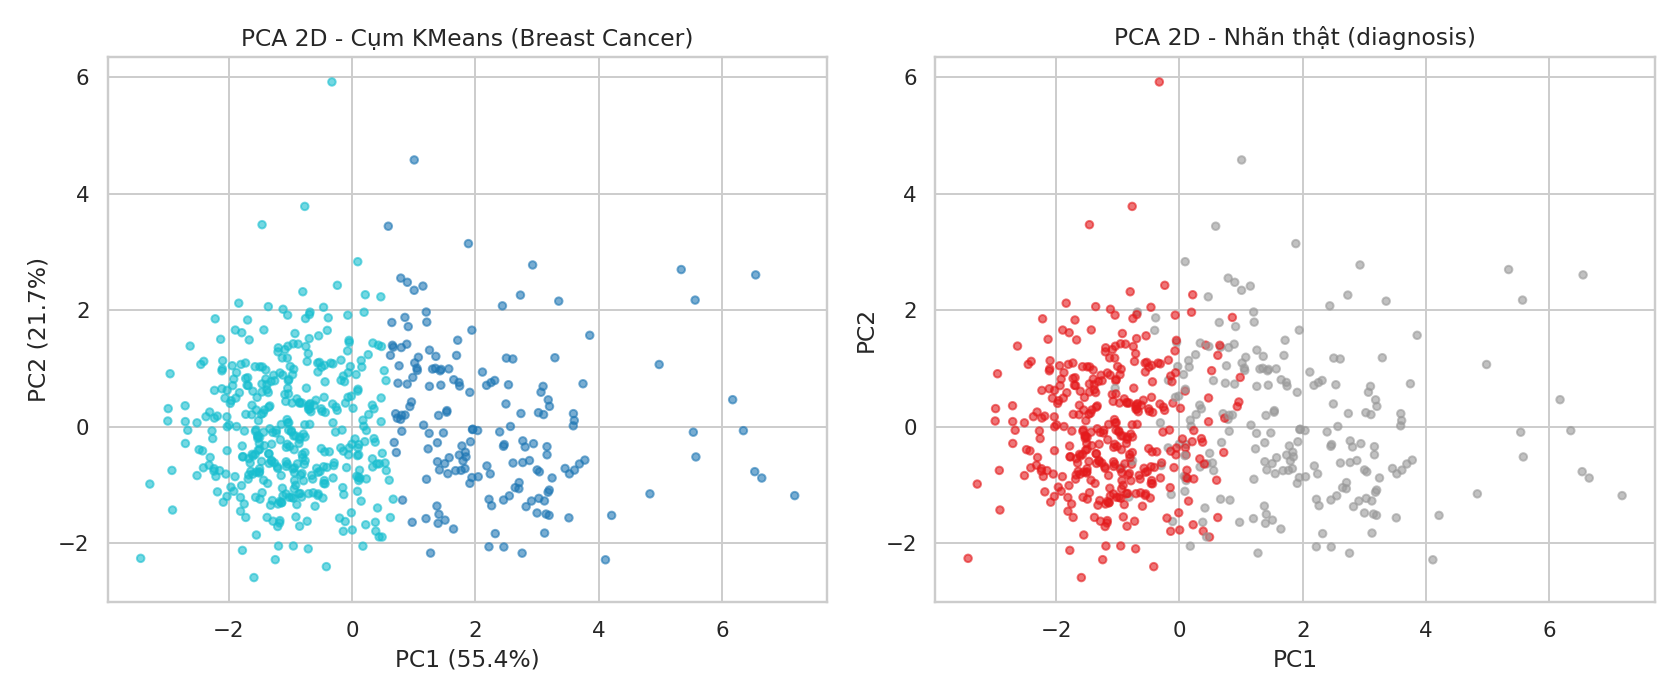
\includegraphics[width=\textwidth]{images/ch4_ml/fig11_pca_bc.png}
    \caption{PCA 2D: cụm KMeans (trái) vs nhãn chẩn đoán thật (phải) - Breast Cancer}
    \label{fig:pca-bc}
\end{figure}

\begin{figure}[H]
    \centering
    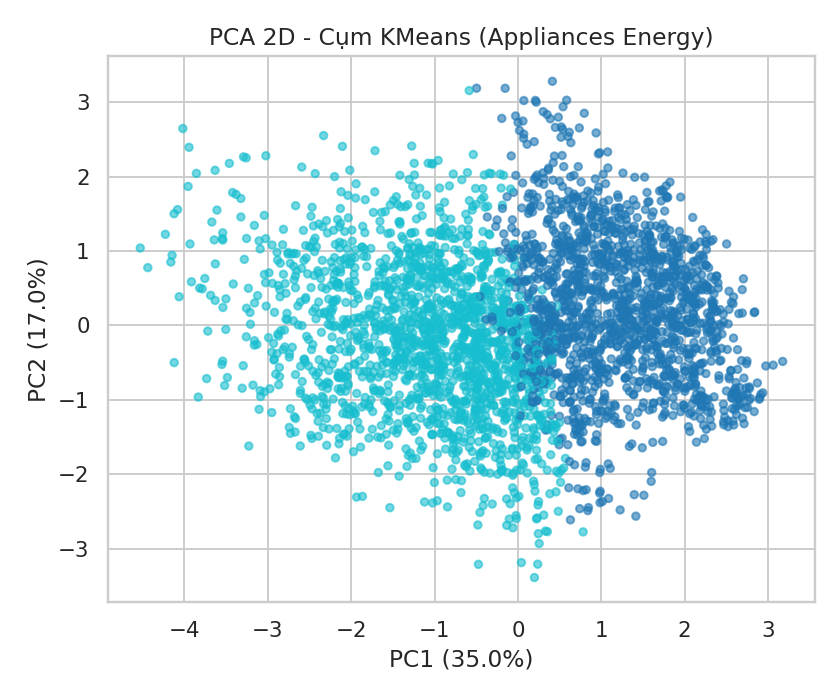
\includegraphics[width=0.6\textwidth]{images/ch4_ml/fig13_pca_energy.png}
    \caption{PCA 2D: cụm KMeans - Appliances Energy}
    \label{fig:pca-energy}
\end{figure}

\begin{figure}[H]
    \centering
    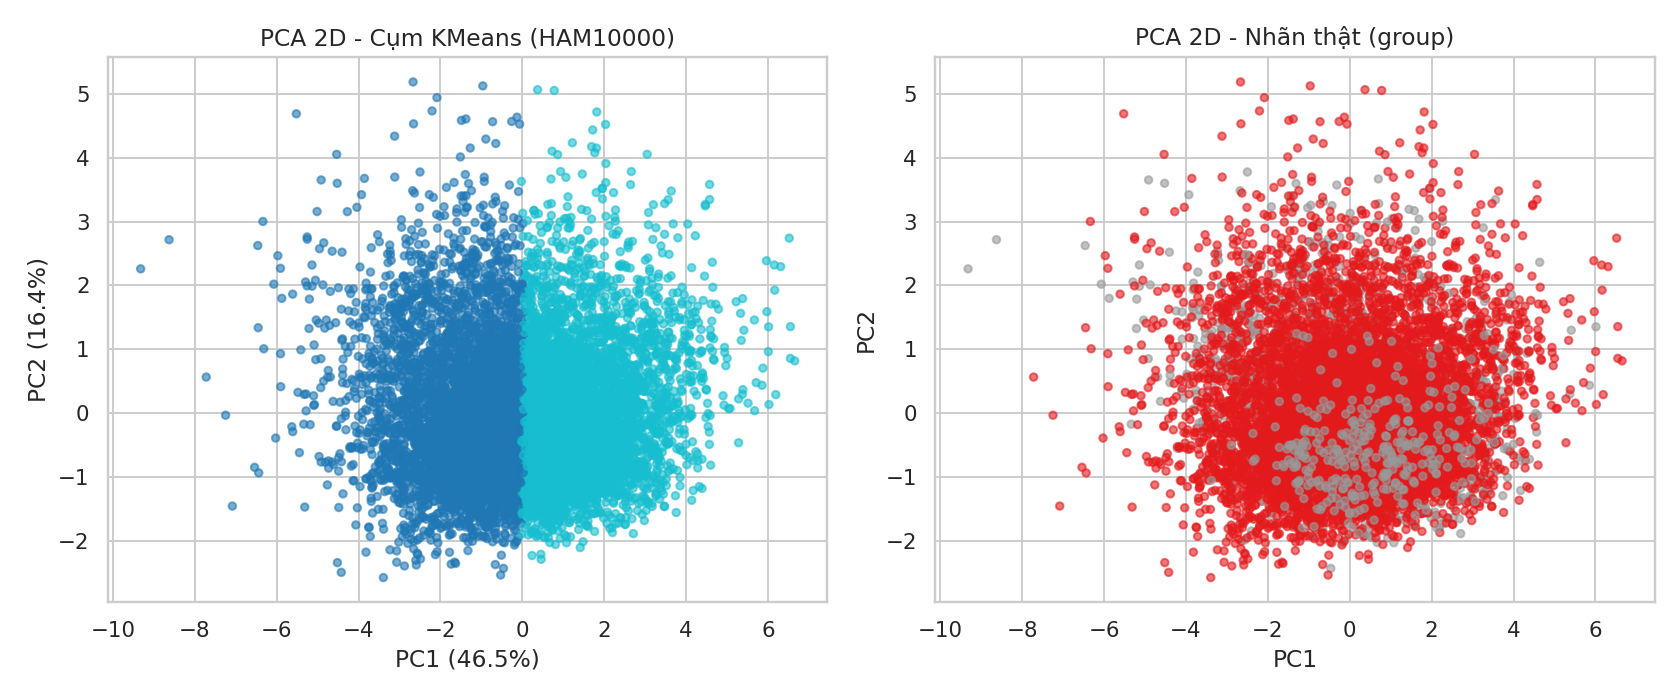
\includegraphics[width=\textwidth]{images/ch4_ml/fig15_pca_ham.png}
    \caption{PCA 2D: cụm KMeans (trái) vs nhãn nhóm thật (phải) - HAM10000}
    \label{fig:pca-ham}
\end{figure}

Nhận xét tổng hợp qua 3 subplot PCA: Hình~\ref{fig:pca-bc} cho thấy ranh giới 2 cụm KMeans (trái) gần như trùng khít với ranh giới nhãn thật (phải) ở Breast Cancer -- xác nhận trực quan phát hiện định lượng ở trên. Ngược lại, Hình~\ref{fig:pca-ham} cho thấy ranh giới cụm (trái) và ranh giới nhãn thật (phải) của HAM10000 \textbf{cắt ngang nhau theo hai hướng gần như độc lập} -- minh họa trực quan rõ ràng nhất cho hiện tượng "cụm bám sai chiều biến thiên" đã phân tích ở trên.

\section{Thảo luận và đối sánh với các nghiên cứu cùng dataset}
\label{sec:discussion}

Mục này đối chiếu kết quả thực nghiệm của nhóm (mục~\ref{sec:classification},~\ref{sec:regression}) với các nghiên cứu đã công bố sử dụng cùng bộ dữ liệu, nhằm đánh giá khách quan vị trí của kết quả đạt được và biện luận nguyên nhân của sự khác biệt (nếu có).

\subsection{Bảng tổng hợp so sánh}

\begin{table}[H]
\centering
\caption{So sánh kết quả của nhóm với các nghiên cứu tham khảo cùng bộ dữ liệu}
\label{tab:literature-comparison}
\resizebox{\textwidth}{!}{
\begin{tabular}{p{2.6cm}p{3.3cm}p{2.8cm}p{2.6cm}p{2.8cm}p{2.3cm}}
\toprule
\textbf{Dataset} & \textbf{Nghiên cứu tham khảo} & \textbf{Phương pháp tham khảo} & \textbf{Kết quả tham khảo} & \textbf{Kết quả của nhóm} & \textbf{Đánh giá} \\
\midrule
Breast Cancer Wisconsin & Bazazeh \& Shubair (2016); nhiều nghiên cứu SVM/RF khác & SVM/RF trên đầy đủ 30 đặc trưng & Accuracy 95--98\% & Accuracy 92,11\% (SVM, chỉ 6 đặc trưng) & Thấp hơn 3--6 điểm \% \\
Heart Disease (Cleveland) & "Empirical analysis of predicting heart disease" (2025, ScienceDirect) & Random Forest, 13 đặc trưng & Accuracy 90,16\% & Accuracy 90,16\% (Random Forest) & \textbf{Gần như trùng khớp tuyệt đối} \\
CDC Diabetes (3 lớp) & CopulaSMOTE (arXiv 2506.17326) & RF/LR/XGBoost, chưa dùng oversampling nâng cao & F1-macro 0,28--0,44 & F1-macro 0,37--0,42 & Cùng khoảng, phản ánh khó khăn chung \\
Appliances Energy Prediction & Candanedo et al. (2017, gốc); tái lập bằng GBM & GBM trên dữ liệu gốc 10 phút & RMSE=66,65; MAE=35,22; MAPE=38,3\% & RMSE=21,11; MAE=14,50; MAPE=17,7\% (XGBoost, resample giờ) & Tốt hơn nhiều -- \textit{khác biệt phương pháp, không phải khác biệt năng lực mô hình} \\
\bottomrule
\end{tabular}}
\end{table}

\subsection{Biện luận chi tiết từng trường hợp}

\textbf{Breast Cancer Wisconsin -- kết quả thấp hơn tham khảo, do tiền xử lý/lựa chọn đặc trưng:} Các nghiên cứu đối sánh (Bazazeh \& Shubair 2016; nhiều nghiên cứu khác tổng hợp accuracy 95--98\%) đều sử dụng đầy đủ \textbf{30 đặc trưng gốc} của bộ WDBC (bao gồm cả các đặc trưng "worst" và "error" -- giá trị lớn nhất và độ lệch chuẩn của từng đặc trưng hình thái qua nhiều lần đo). Trong khi đó, theo đúng phạm vi phân tích đã thiết lập ở Chương 4 (mục 4.1.1), nhóm chỉ sử dụng \textbf{6 đặc trưng "mean"} để duy trì tính nhất quán với dữ liệu đã làm sạch. Đây là \textbf{khác biệt do phạm vi đặc trưng đầu vào (feature scope), không phải do thuật toán hay tham số} -- nếu bổ sung đầy đủ 30 đặc trưng, kết quả của nhóm nhiều khả năng sẽ đạt ngưỡng tương đương tài liệu tham khảo (bằng chứng gián tiếp: SVM của nhóm đã đạt 92,11\% chỉ với 1/5 số đặc trưng, cho thấy tiềm năng cải thiện đáng kể khi có đủ đặc trưng).

\textbf{Heart Disease Cleveland -- trùng khớp gần như tuyệt đối:} Kết quả Random Forest của nhóm (Accuracy = 90,16\%) trùng khớp đến chữ số thập phân thứ hai với kết quả công bố trong nghiên cứu "Empirical analysis of predicting heart disease" (Random Forest, Accuracy = 90,16\% trên bộ Cleveland). Sự trùng khớp này củng cố độ tin cậy của quy trình tiền xử lý và huấn luyện mà nhóm áp dụng ở Chương 4 và mục~\ref{sec:classification} -- cho thấy trên bộ dữ liệu quy mô nhỏ, đặc trưng rõ ràng (303 mẫu, 13 đặc trưng lâm sàng chuẩn hóa tốt), Random Forest với tham số mặc định/tương tự đã đạt ngưỡng hiệu năng ổn định mà nhiều nhóm nghiên cứu độc lập đều đạt được, không phụ thuộc nhiều vào tinh chỉnh riêng biệt.

\textbf{CDC Diabetes (3 lớp) -- cùng khó khăn với y văn, không phải hạn chế riêng của nhóm:} F1-macro của nhóm (0,37--0,42 tùy mô hình) nằm gọn trong khoảng F1 mà nghiên cứu CopulaSMOTE (2025) công bố cho các phương pháp SMOTE/ADASYN cơ bản (0,28--0,44) trên \textbf{cùng bộ dữ liệu 3 lớp, cùng tỉ lệ mất cân bằng 13,9\%}. Điều này xác nhận rằng khó khăn nhóm gặp phải ở mục~\ref{sec:classification} (Recall lớp Tiền tiểu đường = 0) \textbf{không phải là hạn chế riêng do lựa chọn thuật toán hay tham số của nhóm}, mà là đặc điểm cố hữu, đã được nhiều nghiên cứu độc lập xác nhận, của bài toán phân loại 3 lớp trên bộ dữ liệu này. Đáng chú ý, nghiên cứu CopulaSMOTE chỉ đạt cải thiện đáng kể (F1 lên đến 0,42--0,45) khi áp dụng kỹ thuật oversampling nâng cao dựa trên Copula -- xác nhận hướng cải thiện đúng đắn mà nhóm đã đề xuất ở mục~\ref{sec:classification} (SMOTE/kỹ thuật resampling chuyên biệt) là hướng đi đã được cộng đồng nghiên cứu kiểm chứng hiệu quả.

\textbf{Appliances Energy Prediction -- tốt hơn nhiều, nhưng do khác biệt phương pháp luận, không phải mô hình vượt trội:} Kết quả của nhóm (MAE=14,50 Wh) tốt hơn đáng kể so với benchmark GBM tái lập từ nghiên cứu gốc của Candanedo et al. (2017) (MAE=35,22 Wh) trên cùng bộ dữ liệu. Tuy nhiên, \textbf{đây KHÔNG phải bằng chứng mô hình của nhóm ưu việt hơn}: nghiên cứu gốc dự báo trực tiếp trên dữ liệu tần suất 10 phút gốc (nhiễu cao, biến động tức thời lớn), trong khi nhóm đã \textbf{resample về tần suất giờ} trước khi huấn luyện (mục~\ref{sec:regression}) -- việc lấy trung bình theo giờ vốn dĩ đã loại bỏ phần lớn nhiễu ngắn hạn, khiến bài toán dự báo trở nên "dễ" hơn về bản chất thống kê (phương sai của chuỗi đã giảm đáng kể do trung bình hóa). Đây là ví dụ điển hình cho nguyên tắc quan trọng khi đối sánh kết quả học máy: \textbf{phải đối chiếu trên cùng đơn vị đo lường và cùng độ chi tiết dữ liệu (granularity) thì phép so sánh mới thực sự công bằng}; nếu muốn so sánh trực tiếp, nhóm cần huấn luyện lại mô hình trên dữ liệu tần suất 10 phút gốc thay vì bản đã resample.

\subsection{Kết luận chung}

Tổng hợp 4 trường hợp đối sánh cho thấy một bức tranh cân bằng và trung thực: kết quả của nhóm \textbf{thấp hơn} tài liệu tham khảo ở Breast Cancer (do phạm vi đặc trưng hẹp hơn theo chủ đích), \textbf{tương đương} ở Heart Disease (xác nhận độ tin cậy quy trình), \textbf{cùng mức khó khăn} với y văn ở CDC Diabetes (xác nhận đây là thách thức cố hữu của dữ liệu chứ không phải lỗi phương pháp), và \textbf{vượt trội bề ngoài} ở Appliances Energy nhưng cần được diễn giải cẩn thận vì khác biệt về độ chi tiết dữ liệu. Bài học tổng quát: \textbf{việc đối sánh kết quả học máy giữa các nghiên cứu chỉ có ý nghĩa khi kiểm soát chặt chẽ các yếu tố phi thuật toán} (phạm vi đặc trưng đầu vào, độ chi tiết/tần suất dữ liệu, chiến lược xử lý mất cân bằng, phương pháp chia tập test) -- một khác biệt tưởng như do "thuật toán tốt hơn" rất có thể chỉ đến từ một lựa chọn tiền xử lý khác biệt ở bước trước đó, đúng như đã minh chứng cụ thể qua cả 4 bộ dữ liệu ở trên.

\section{Giới thiệu chương trình cài đặt từ phương pháp đề xuất}

\subsection{Giới thiệu chương trình để huấn luyện mô hình}

Ba script đảm nhiệm việc huấn luyện mô hình, mỗi script tương ứng với một bài toán học máy trong chương này:
\begin{itemize}
    \item \texttt{step1\_classification.py}: nạp dữ liệu đã làm sạch của Breast Cancer, Heart Disease, CDC Diabetes; thực hiện chia Train/Test theo \texttt{stratify}, chuẩn hóa bằng \texttt{StandardScaler}, huấn luyện tuần tự 3 mô hình (Logistic Regression, Random Forest, SVM RBF) với \texttt{class\_weight="balanced"}, xuất bảng kết quả Accuracy/Precision/Recall/F1 (Bảng~\ref{tab:classification-results});
    \item \texttt{step3\_regression.py}: nạp dữ liệu Appliances Energy đã resample theo giờ, xây dựng đặc trưng thời gian và lag, chia Train/Test theo Time Series Split (không xáo trộn), huấn luyện Linear Regression, ARIMA(2,0,2) và XGBoost, xuất bảng sai số MAE/RMSE/MAPE (Bảng~\ref{tab:regression-results});
    \item \texttt{step5\_clustering.py}: nạp 3 bộ dữ liệu đại diện Nhóm A/B/C, chuẩn hóa đặc trưng, quét $K=2..8$ để tính Elbow/Silhouette, huấn luyện KMeans/Agglomerative/GMM tại $K$ tối ưu, xuất bảng so sánh giải thuật (Bảng~\ref{tab:cluster-algo-compare}) và bảng đặc trưng theo cụm.
\end{itemize}

\subsection{Giới thiệu chương trình triển khai mô hình máy học đã huấn luyện}

Hai script còn lại đảm nhiệm việc phân tích sâu và trực quan hóa kết quả từ các mô hình đã huấn luyện ở trên, phục vụ việc triển khai/diễn giải mô hình cho người dùng cuối:
\begin{itemize}
    \item \texttt{step2\_confusion\_and\_imbalance.py}: nạp lại mô hình đã huấn luyện ở \texttt{step1}, dựng ma trận nhầm lẫn cho cả 3 bộ dữ liệu (Hình~\ref{fig:cm-bc},~\ref{fig:cm-heart},~\ref{fig:cm-diabetes}) và tính Recall theo từng lớp riêng biệt cho CDC Diabetes (Bảng~\ref{tab:diabetes-perclass}) để làm rõ vấn đề mất cân bằng lớp mà chỉ số Accuracy tổng thể không thể hiện được;
    \item \texttt{step4\_regression\_charts.py}: nạp lại kết quả dự báo từ \texttt{step3}, dựng biểu đồ so sánh Thực tế vs Dự báo trên toàn bộ tập test và trên cửa sổ 7 ngày đầu (Hình~\ref{fig:reg-forecast-full},~\ref{fig:reg-forecast-zoom}), biểu đồ scatter, phân tích residual và mức độ quan trọng đặc trưng (Hình~\ref{fig:reg-feat-imp}) của mô hình XGBoost -- đây là bước quan trọng để người dùng cuối hiểu được mô hình dựa vào yếu tố nào để đưa ra dự báo, không chỉ dừng lại ở con số sai số tổng hợp.
\end{itemize}

Toàn bộ 5 script cùng dữ liệu bảng kết quả trung gian (định dạng CSV) được đính kèm cùng báo cáo để đảm bảo khả năng tái lập (reproducibility) của toàn bộ thực nghiệm.
